% \documentclass{article}
% \usepackage{xeCJK}
% \usepackage{tikz}
% \usetikzlibrary{decorations.pathreplacing, calligraphy}
% \usetikzlibrary{quotes,angles}
% \begin{document}
\begin{tikzpicture}
    \node at (0,0) {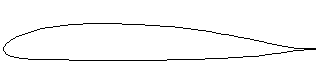
\includegraphics[width = 4cm, angle = -30]{OA212.png}};
    \draw[-latex](-0.5,0.2)--(-2.5,0.2) node[below]{$Y_{bl}$};
    \draw[-latex](-0.5,0.2)--(-0.5,2) node[left]{$Z_{bl}$};
    \draw[-latex](-0.5,0.2)--(-2.5,1.2) node[above]{$X_{el,i}$};
    \draw[-latex](-0.5,0.2)--(-1.1,-1.2) node[left]{$Z_{el,i}$};
    \draw 
    (-2.5,1.2)coordinate(a)
    (-0.5,0.2)coordinate(b)
    (-2.5,0.2)coordinate(c)
    pic["$\theta_{el,i}$", draw=orange, <-, angle eccentricity=1.2, angle radius=1.5cm]
    {angle=a--b--c};

\end{tikzpicture}  

% \end{document}